\documentclass{article}
\usepackage{graphicx}
\usepackage{amsmath}
\usepackage{amssymb}
\usepackage[italicdiff]{physics}
\usepackage{enumerate}
\usepackage{microtype}
\DisableLigatures{encoding= *, family=*}
\usepackage{titlesec}
\usepackage{xfrac}
\setcounter{secnumdepth}{4}
\usepackage{xcolor}
\usepackage[bookmarks=false]{hyperref}
\usepackage{mathtools}
\hypersetup{
    colorlinks=true,
    linkcolor=[RGB]{59 108 209},
    urlcolor=[RGB]{59 108 209}
}
\urlstyle{same}

\titleformat{\paragraph}
{\normalfont\normalsize\bfseries}{\theparagraph}{1em}{}
\titlespacing*{\paragraph}
{0pt}{3.25ex plus 1ex minus .2ex}{1.5ex plus .2ex}

\title{Determinants}
\author{}
\date{}

\begin{document}
\maketitle

\section{Definition of Determinants}

Let\begin{equation*}
    \begin{cases}
        a_{1}x+b_{1}y=0 \\
    a_{2}x+b_{2}y=0
    \end{cases}
\end{equation*}

Solving for $\dfrac{y}{x}$ we get, 

$$\dfrac{y}{x}=-\dfrac{a_{1}}{b_{1}}=-\dfrac{a_{2}}{b_{2}} \implies \dfrac{a_{1}}{b_{1}}=\dfrac{a_{2}}{b_{2}}$$

The quantity $a_{1}b_{2}-a_{2}b_{1} $ is represented by $\begin{vmatrix}
    a_{1} & b_{1} \\
    a_{2} & b_{2}
\end{vmatrix}$

Also, for\begin{equation*}
    \begin{cases}
        a_{1}x+b_{1}y+c_{1}z=0 \\
        a_{2}x+b_{2}y+c_{2}z=0 \\
        a_{3}x+b_{3}y+c_{3}z=0
    \end{cases}
\end{equation*}
$$\therefore \begin{vmatrix}
    a_{1} & b_{1} & c_{1} \\
    a_{2} & b_{2}&c_{2} \\
    a_{3} &b_{3} &c_{3} 
\end{vmatrix}=a_{1}\left(b_{2}c_{3} - b_{3}c_{2} \right)-b_{1}\left(a_{2}c_{3}-c_{2}a_{3} \right)+c_{1}\left(c_{3}a_{2}-c_{2}a_{3} \right) $$

\begin{itemize}
    \item $\text{A determinant of $n$th order consists of $n!$ terms in its expansion.}$
    \item $\text{Shape of Every Determinant is a square.}$
\end{itemize}

\section{Sarrus Rule of Determinant Expansion}
Let, $$\Delta = \begin{vmatrix}
    a_{1} &b_{1} &c_{1} \\
     a_{2} &b_{2} &c_{2} \\
     a_{3} &b_{3} &c_{3}  
\end{vmatrix}$$
Write down the three rows of $\Delta$ and rewrite the first two rows. 

\begin{center}
    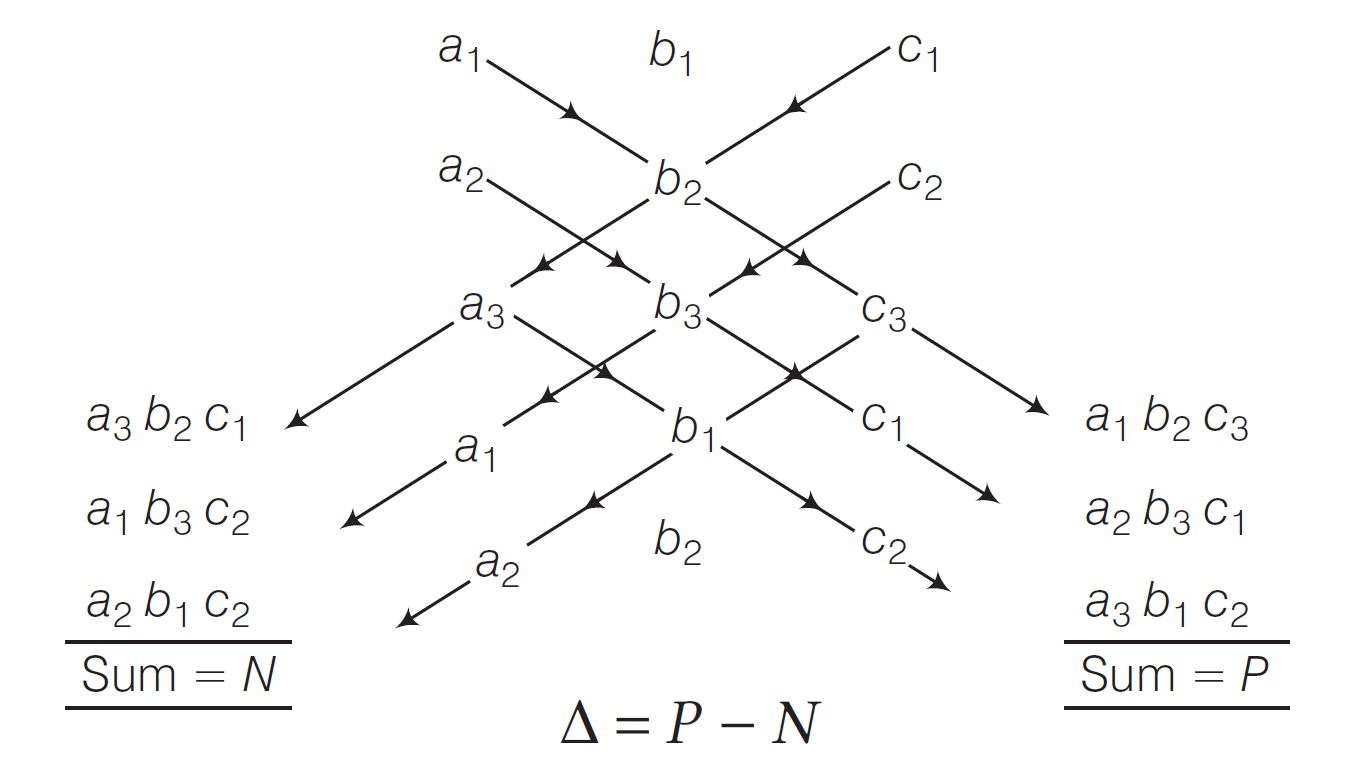
\includegraphics[scale=0.3]{img_1.png}
\end{center}
\section{Window Rule}
Consider, $$\Delta = \begin{vmatrix}
    a_{1} &b_{1} &c_{1} \\
     a_{2} &b_{2} &c_{2} \\
     a_{3} &b_{3} &c_{3}  
\end{vmatrix}$$

\begin{center}
    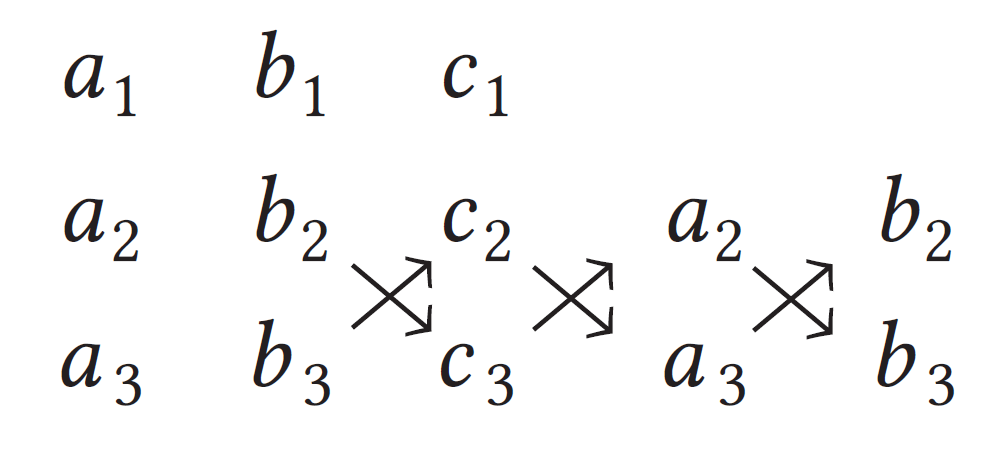
\includegraphics[scale=0.2]{img_2.png}
\end{center}
$\Delta = a_{1}\left(b_{2}c_{3} - b_{3}c_{2} \right)-b_{1}\left(a_{2}c_{3}-c_{2}a_{3} \right)+c_{1}\left(c_{3}a_{2}-c_{2}a_{3} \right)$

\section{Minors and Cofactors}

Let $$\Delta = \begin{vmatrix}
    a_{11} & a_{12} & a_{13} & \ldots & a_{1n} \\
    a_{21} & a_{22} & a_{23} & \ldots & a_{2n} \\
    a_{31} & a_{32} & a_{33} & \ldots & a_{3n} \\
    \vdots & \vdots & \vdots& \ddots & \vdots \\
    a_{n1} & a_{n2} & a_{n3} & \ldots & a_{nn}
\end{vmatrix}\hspace{2cm} \forall  \hspace{2mm} n \in \mathbb{N}-\left\{1\right\}$$
The determinant of order $n-1$ obtained from $\Delta$ after deleting $ith $ row and $jth $ column is called the $\textit{Minor of $a_{ij}$}$ (Denoted by $M_{ij}$) \\

Cofactor of $a_{ij}=C_{ij}=(-1)^{i+j} \cdot M_{ij} $

\subsection{Important Results for Cofactors}
\begin{enumerate}[1.]
    \item $\Delta =a_{11}C_{11}+a_{12}C_{12}+ \ldots +a_{nn}C_{nn}=\displaystyle\sum_{r=1}^{n} a_{\omega r}C_{\omega r} \hfill \omega \in \mathbb{N}$
    \item The sum of the product of an element of any row (or column)
with corresponding cofactors of another row (or column) is
equal to zero.

$a_{11}C_{21}+a_{12}C_{22}+\ldots + a_{1n}C_{2n}= \displaystyle\sum_{r=1}^{n} a_{\omega r}C_{(\omega +1)r}=0 \hfill \omega \in \mathbb{N}-\left\{n\right\}$

\item $\Delta ^c=\Delta ^{n-1}, \Delta ^c \text{ is determinant made by cofactors of elements in $\Delta$}$

For 3rd order determinant $\Delta^c=\Delta ^2$
\end{enumerate}
\section{Use of Determinants in Coordinate Geometry}
\begin{enumerate}[1.]
    \item Area of Triangle whose vertices are $(x_{1},y_{1}), (x_{2},y_{2}),(x_{3},y_{3}) $ is 
    $$\dfrac{1}{2} \abs{\begin{vmatrix}
        x_{1} & y_{1} & 1 \\
        x_{2} & y_{2} & 1 \\
        x_{3} & y_{3} & 1
    \end{vmatrix}}$$
    \item If $a_{i}x+b_{i}y+c_{i}=0, i \in \left\{1,2,3\right\} $ are the sides of a triangle, then the area of triangle is 
    $$\dfrac{1}{\abs{2C_{1}C_{2}C_{3}}}\begin{vmatrix}
        a_{1} & b_{1} & c_{1} \\
        a_{2} & b_{2} & c_{2} \\
        a_{3} & b_{3} & c_{3} 
    \end{vmatrix}^2 \hfill $$
\end{enumerate}
\end{document}
